\newpage

\section{Temporal and geographical components}

Using the proposed model, the first step is to understand the main component of the commuting dynamic. The result of our approach will emerge from this main component as we can see in the next picture. This main component model the first logic result and shows the time segments that people have more activite, in call numbers terms. This picture shows static and dinamic users calling i.e.: nodes with self-edges are counted and transition edges together.

\begin{figure}[ht]
\centering
\subfigure[Total number of calls grouped by Week days]{
	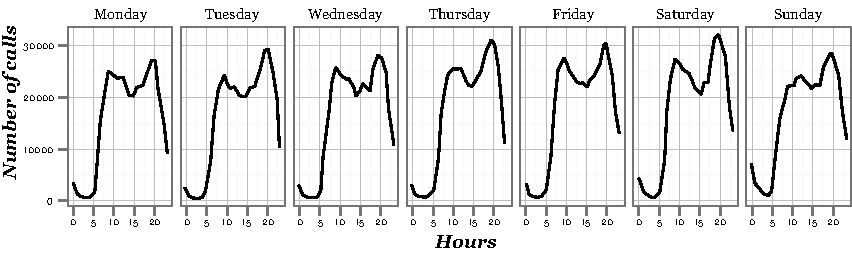
\includegraphics[scale =0.5] {results/images/calls_number.pdf}
	\label{fig:subfig11}
}
\label{fig:fig1}
\end{figure}

As the above picture shows, we can see two peaks $p_1$ from 7 Am to 9 Am and another one $p_2$ from 6 Pm to 8 Pm. As we can see $p_1 < p_2$ in a number of call terms and $p_2$ start to grow at 6 PM and get its maximum value at 8 PM, after this hour, the number of calls dicrease linearly. Another main thing showed by the picture is that exists a central valley between $p_1$ and $p_2$, i.e.:  from 9 Am to 6 Pm, that people stop or "relax??" the number of calls. 
This main component is common to the seven days of the week, therefore, we can assume that people have the same behavior on this sample dataset.
\\
\\
\\
\\
Several assumptions could be suggested at this point, for instance, in the $p_1$ range, people start to work on a regular daily activite, in the central valley, some people stop (but not entirely), perhaps to eat, and in the next peak $p_2$, people return to regular daily activite and perhaps start to return home.
The question here is to figure out the commuting dynamic through the average displacement per person and where are located the time ranges or windows that people realize this action.  This last assumption, will be tested with the proposed model and the final GIS visualization as main core of the work showed by thw present work.  Geographical displacements are studied by means of GIS tool on the map in order to detect and understand the micro and long movements across the country. 
\\
\\
A pattern model of commuting is showed as a start point to test the hypothesis. {\color{red} Poner algunas referencia or something del supuesto modelo teórico!!}. As we can see two peaks are defined corresponding with maximum displacement hours and a central valley corresponding to "eat hours"  {\color{red} queda poco científico, hay que poner algo mejor}

\newpage

\setcounter{subfigure}{0}
\begin{figure}[h]
\begin{center}
$\begin{array}{cc}
\subfigure{
	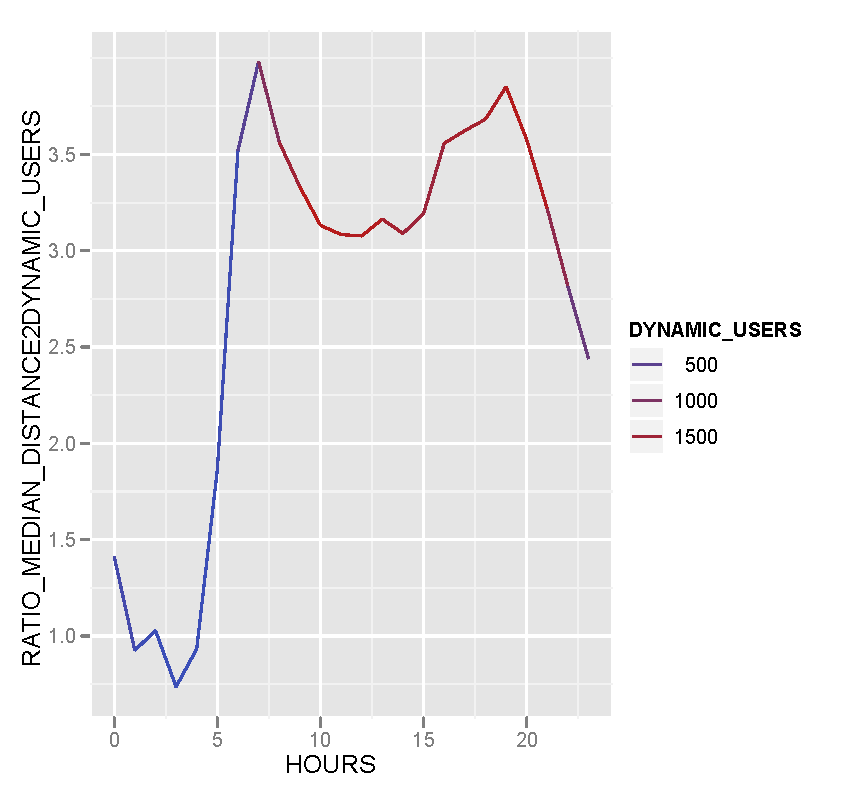
\includegraphics[scale =0.5] {results/images/monday_commuting_lenght.pdf}
	\label{fig:subfig11}
}
\label{fig:fig1}
\end{array}$
\end{center}
\caption{Theoretical Commuting Model (cambiar por la imagen de verdad)}
\end{figure}

The picture above, shows a first approach pattern model of commuting. Two peaks representing high displacement temporal events are modeled with a central valley.   {\color{red} Escribir mas sobre el porque de este modelo teorico, porque la eleccion de los dos picos y del valle central.}
\\
\\
Datasets has been processed carried out by the mathematical model proposed, therefore, static users has been removed and dinamyc users, better its tracks, has been grouped into a temporal windows and grouped by the day of the week. Seven pictures representing the 24 hours of each day are shown below in and their respective data tables. The median normalized with the number of dynamic users, is showed in each temporal window of each picture corresponding with each day of the week.
\\
\\
Pictures shows that emerge a new $p'_1$ and $p'_2$ where $p'_1 > p'_2$, in a displacements terms, we can see that people start to perform moves about 4 AM until to reach $p'_1$ at 7 Am. At this point, displacements are reduced 

\setcounter{subfigure}{0}
\begin{figure}[h]
\begin{center}
$\begin{array}{cc}

\subfigure[Monday]{
	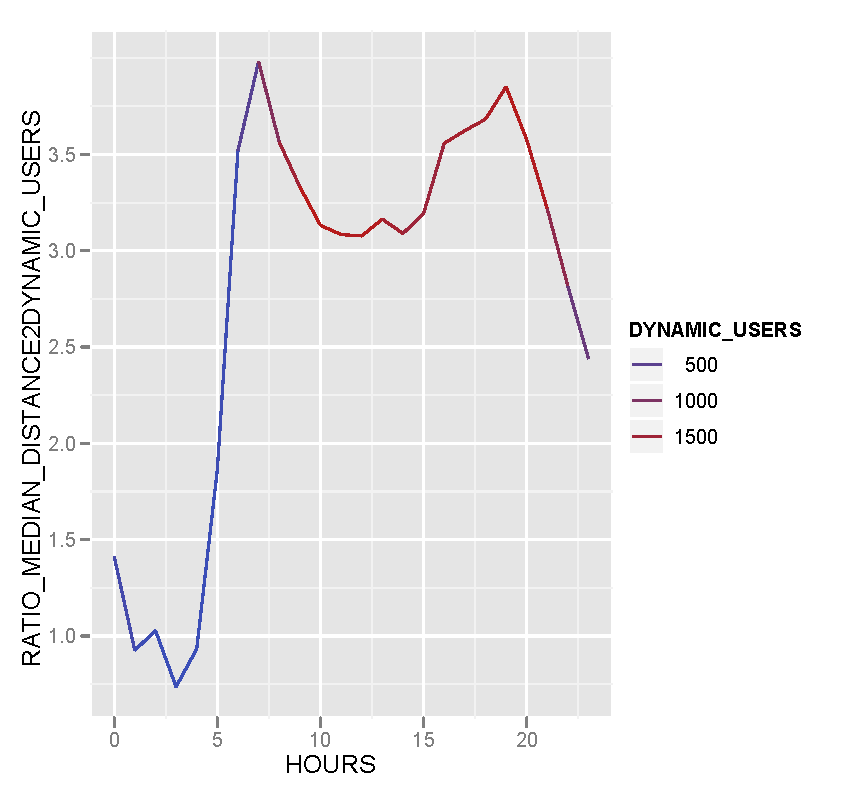
\includegraphics[scale =0.5] {results/images/monday_commuting_lenght.pdf}
	\label{fig:subfig11}
}
\label{fig:fig1}
 &
\subfigure[Thuesday]{
	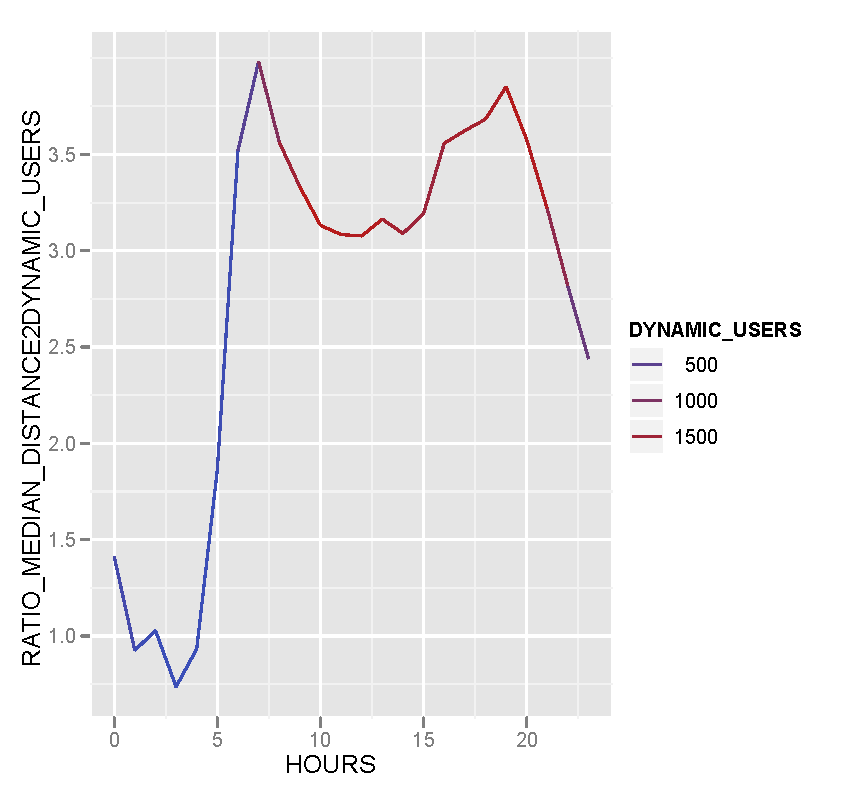
\includegraphics[scale =0.5] {results/images/monday_commuting_lenght.pdf}
	\label{fig:subfig11}
}
\label{fig:fig1}
\\
\subfigure[Wednesday]{
	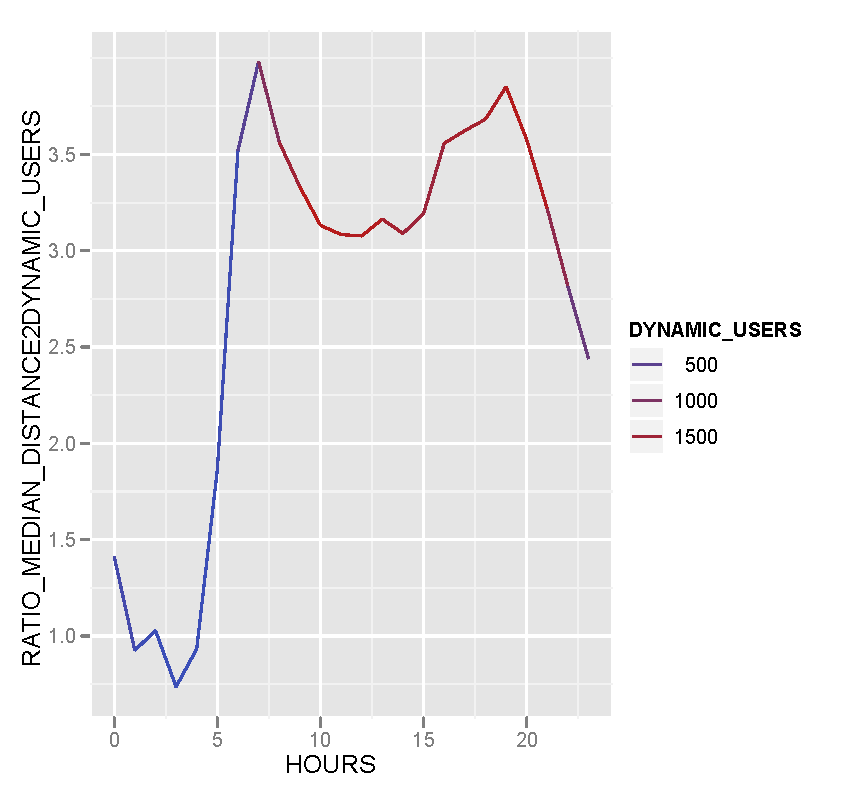
\includegraphics[scale =0.5] {results/images/monday_commuting_lenght.pdf}
	\label{fig:subfig11}
}
\label{fig:fig1}
&
\subfigure[Thursday]{
	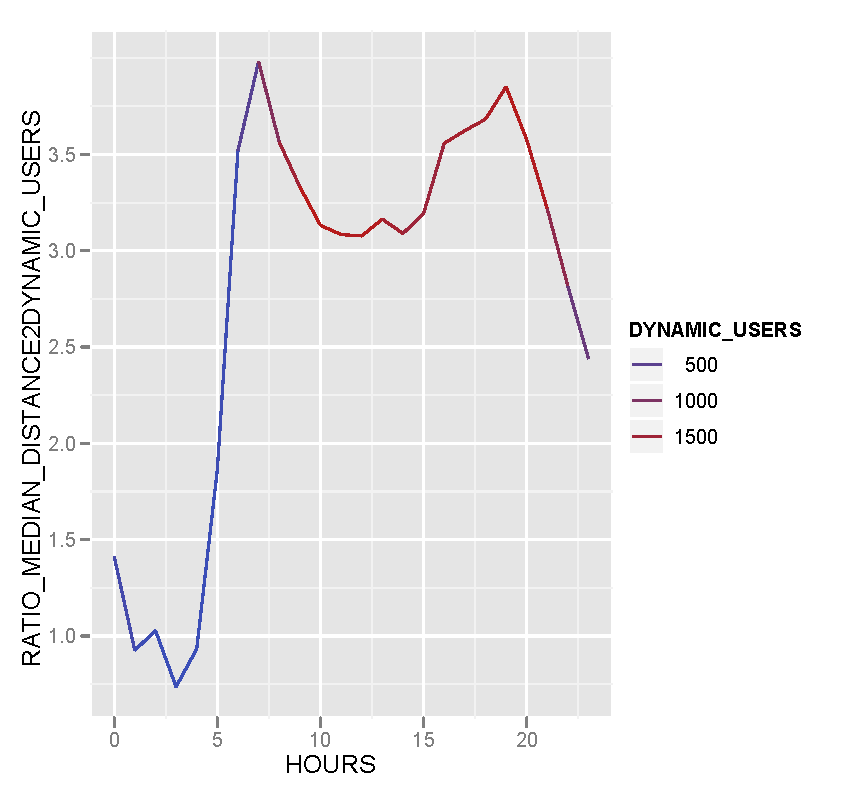
\includegraphics[scale =0.5] {results/images/monday_commuting_lenght.pdf}
	\label{fig:subfig11}
}
\label{fig:fig1}
\\
\subfigure[Friday]{
	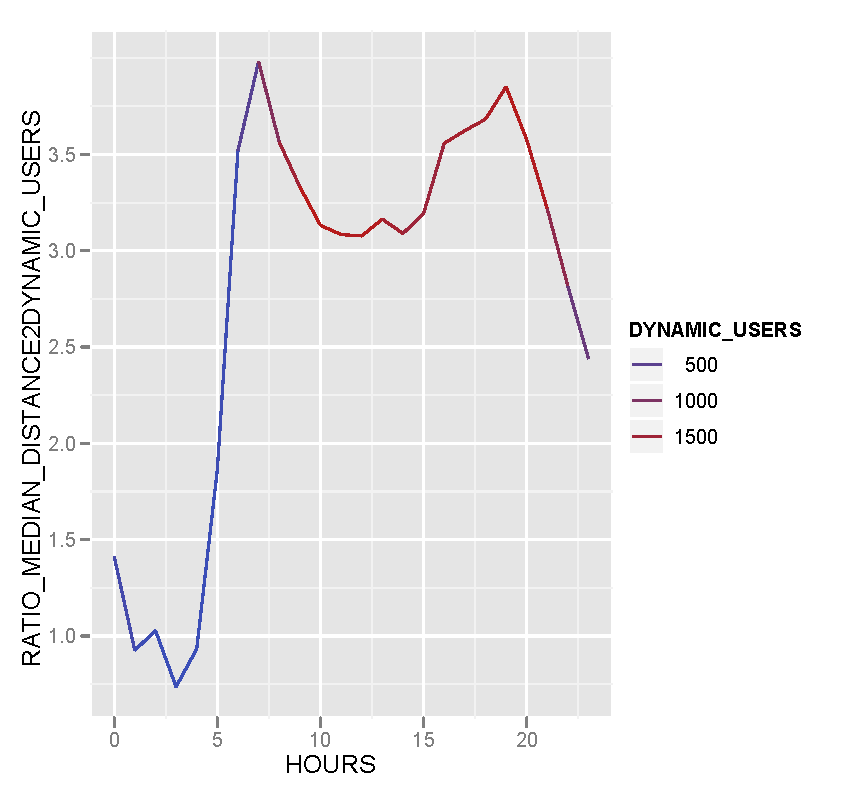
\includegraphics[scale =0.5] {results/images/monday_commuting_lenght.pdf}
	\label{fig:subfig11}
}
\label{fig:fig1}
 &
\subfigure[Saturday]{
	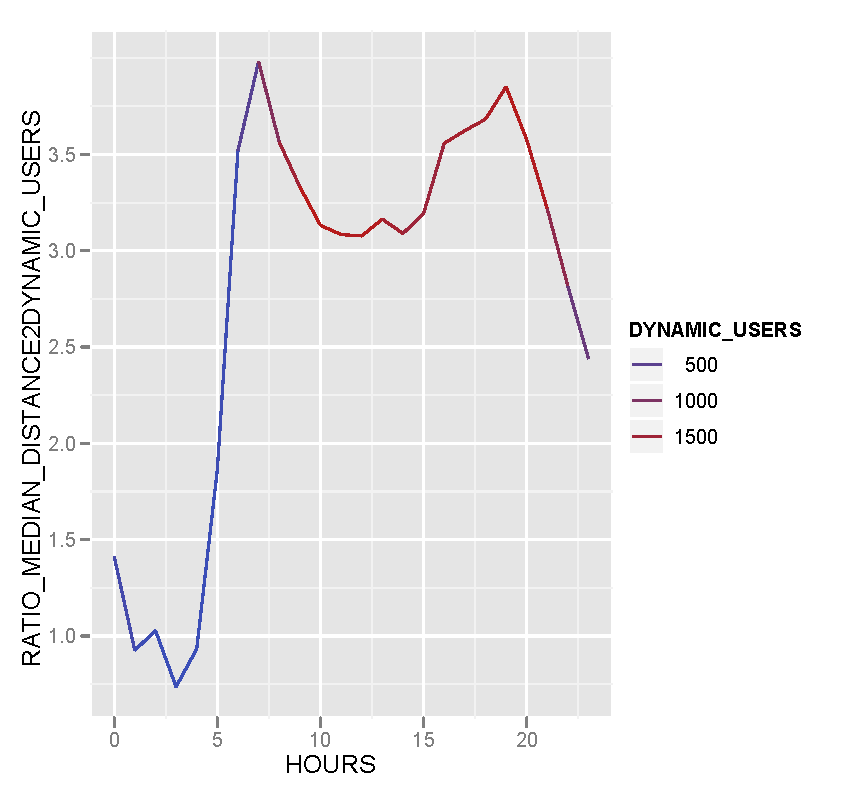
\includegraphics[scale =0.5] {results/images/monday_commuting_lenght.pdf}
	\label{fig:subfig11}
}
\label{fig:fig1}


\end{array}$
\end{center}
\caption{Dynamic users displacment}
\end{figure}




